\newpage
\section{Grundlagen der Kryptographie}
\subsection{Grundbegriffe}
Die folgende grundlegende Erklärung der Grundbegriffe der Kryptographie ist
geschrieben in Anlehnung an Brinkmann, Kapitel 1.1. \par Zu der \gls{kryptographie},
der Kunst Nachrichten oder Daten durch Verschlüsselung geheim zu halten, gibt es
noch andere Wissenschaften, die sich mit Verschlüsselungen befassen. Bei der
Kryptographie werden Nachrichten so unlesbar gemacht, dass sie nur von Empfängern
mit einem geheimen Schlüssel wieder in den ursprünglichen Text umgewandelt werden
können.

\par Parallel zu der Kryptographie gibt es die \gls{steganographie},
bei der die bloße Existenz der zu versteckenden Informationen verborgen wird. Dies
wird dadurch ermöglicht, dass die geheimen Informationen in anderen, harmlos aussehenden
Nachrichten versteckt werden, sodass sie nur von Eingeweihten entdeckt werden
können.

\par Die \gls{kryptoanalyse} befasst sich, entgegen der Kryptographie,
nicht mit der Verschlüsselung, sondern damit, verschlüsselte Nachrichten und
kryptographische Verfahren zu analysieren. Dies wird mit dem Ziel gemacht,
Verschlüsselungen zu brechen.

\par Die Wissenschaft, die Kryptographie und Kryptoanalyse vereint, ist die
\gls{kryptologie}. Diese wird das Kernthema dieser Arbeit sein. \autocite[\pagef~5]{brinkmann_vak_2001}

\subsection{Historische Entwicklung und grundlegende Konzepte}
Besonders in Zeiten des Krieges war es vonnöten, Informationen sicher von den Befehlshabern
zu den Offizieren überbringen zu können. So wurden die ersten kryptographischen
Konzepte für den militärischen und politischen Nutzen entwickelt. \autocite[]{beutelspacher_kurze_2017}

\par Eine grundlegende Erfindung für das Voranschreiten der Kryptographie war die Erfindung des Schlüssels, wobei die Erfindung des variablen Schlüssels die Geburtsstunde der Kryptographie markiert. \autocite[]{beutelspacher_kurze_2017}. Durch variable Schlüssel ist es nun möglich, einfach zwischen verschiedenen Verschlüsselungen zu wechseln.

% \par
\subsubsection{Caesar-Scheibe}\label{subsubsec:caesar-chiffre}
Bei der Caesar-Scheibe (auch Caesar-Chiffre genannt) werden die Buchstaben des Alphabetes
um einen bestimmten Wert, dem Wert des Schlüssels, rotiert. Dabei wird das 'z' als Buchstabe vor dem 'a' gesehen. 

Dieser Schlüssel ändert sich nicht für kommende Zeichen, sondern ist für die gesamte Nachricht identisch. 

\par \autoref{fig:caesarChiffre} verbildlicht die Caesar-Chiffre anhand der klassischen Darstellung zweier konzentrischen Kreise mit dem Schlüssel $13$.
\begin{figure}[htbp]
	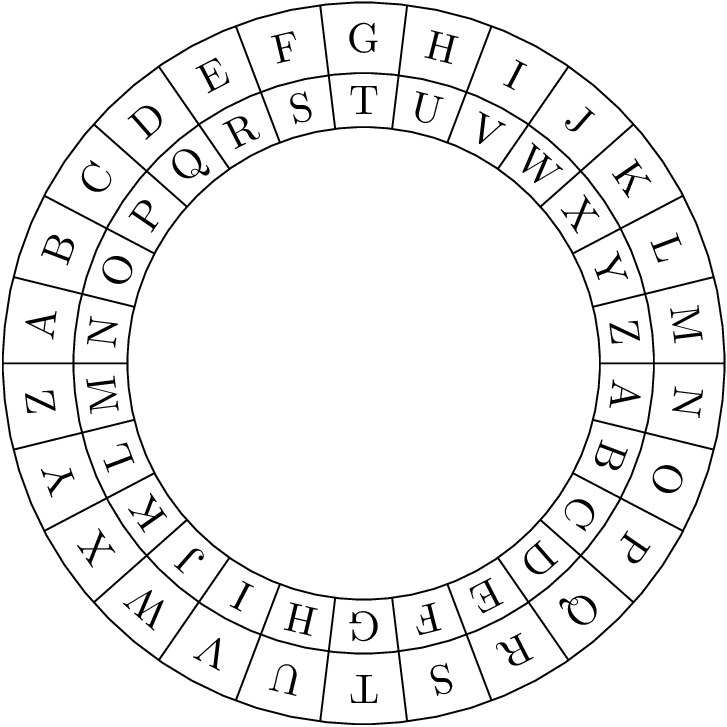
\includegraphics[width=0.6\textwidth]{abbildungen/caesar-chiffre}
	\centering
	\caption[
	Caesar-Chifre am Beispiel einer Scheibe]{Caesar-Chiffre am Beispiel eines Scheibe (Eigene Darstellung)}
	\label{fig:caesarChiffre}
\end{figure}

Caesar hat für seine Verschlüsselungen immer den Schlüssel 3 genutzt \autocite[]{beutelspacher_kurze_2017}, sodass aus CAESAR folglich FDHVDU wird. 
Dies bietet allerdings praktisch keine Sicherheit, besonders nicht nach heutigen Standards.

\par Da es sich durch die Jahrtausende hinweg sich immer wieder gezeigt hat, dass
es fast unmöglich ist, \glspl{algorithmus} geheim zu halten, kam mit der Zeit
die Sorge auf, dass „[wer] das Verfahren kennt, insbesondere wer es erfunden hat,
[…] es auch brechen [kann].“ \autocite{beutelspacher_kurze_2017}. Der Kryptologe Auguste
Kerckhoffs formulierte 1833 in seinem zweiten der sechs Grundsätze zur Konstruktion
eines sicheren Verschlüsselungsferfahrens, dass das System keine Geheimhaltung erfordern darf und ohne Schaden in die Hände von Feinden fallen können. \autocite[Übersetzt aus dem Französischen]{petitcolas_information_nodate}
\subsubsection{Polyalphabetische Codes}
Um 1500 wurde klar, dass \gls{monoalphabetisch}e Codes keine wirkliche
Sicherheit bieten. Im 16. Jahrhundert geschah ein Umdenken in der Verschlüsselung.
Mehrere gelehrten hatten eine ähnliche Idee für eine neue Dimension dieser. \autocite[]{beutelspacher_kurze_2017}
Eines der bekanntesten polyaplhabetischen Verfahren ist die Vigenère-Chiffre, benannt
nach ihrem Entwickler, \textbf{Blaise de Vigènere}.

Bei der Vigènere-Chiffre wird sich, entgegen zu der Caesar-Chiffre, dargestellt in \autoref{subsubsec:caesar-chiffre}, ein Schlüsselwort
überlegt. Sollte dieses Wort kürzer sein, als der eigentliche Text, wird es so
lange wiederholt, bis jedem Zeichen im Klartext ein Zeichen des Schlüssels zugeordnet
ist. Anschließend wird jedes Zeichen im Klartext um das dazu assoziierte Zeichen
des Schlüssels verschoben, sodass für jedes Zeichen ein anderes Zeichen im verschlüsselten
Text herauskommt.

\autoref{tab:vigenere}\autocite[\pagef 6]{kryptographische_algorithmen} zeigt das Vigènere-Verfahren mit dem Schlüssel \enquote{ALICE} auf dem Klartext \enquote{DIES IST EIN VERSCHLÜSSELTER TEXT}

\begin{table}[htbp]
	\resizebox{\textwidth}{!}{%
	\begin{tabular}{l|llllllllllllllllllllllllllllllllll}
		Klartext             & D & I & E & S &  & I & S & T &  & E & I & N &  & V & E & R & S & C & H & L & U & E & S & S & E & L & T & E & R &  & T & E & X & T\\
		\hline
		Schlüssel (Alice)    & A & L & I & C &  & E & A & L &  & I & C & E &  & A & L & I & C & E & A & L & I & C & E & A & L & I & C & E & A &  & L & I & C & E\\
		\hline
		Verschlüsselter Text & D & T & M & U &  & M & S & E &  & M & K & R &  & V & P & Z & U & G & H & W & C & G & W & S & P & T & V & I & R &  & E & M & Z & W\\
		\hline
	\end{tabular}%
	}
	\caption[
	Verschlüsselung mit Vigènere-Verfahren]{Verschlüsselung mit Vigènere-Verfahren\footnotemark}
	\label{tab:vigenere}
\end{table}

\footnotetext{\cite[S. 6]{kryptographische_algorithmen}}

Durch diese nicht gleichmäßige Verschiebung bietet die Vigènere-Chiffre gegenüber der Caesar-Chiffre eine deutlich sicherere Verschlüsselung, ist aber allemal nicht vollständig sicher. Sobald der Schlüssel bekannt ist, muss nur jedes Zeichen des verschlüsselten Textes in entgegengesetzter Richtung des Schlüssels verschoben werden.
\par Dennoch sind polyalphabetische Verschlüsselungsverfahren in Anbetracht der einfachen Durchführung stark und bieten ein großes Potenzial.
\subsubsection{Enigma}
Der Beginn des 20.\ Jahrhunderts läutete die Blütezeit der kryptografischen Maschinen ein.
Diese wurden mit wachsender Komplexität der Verschlüsselungen immer notwendiger.
Die wohl berühmteste Chiffriermaschine der Welt, die Enigma, wurde 1918 von ihrem Erfinder \textbf{Arthur Schebius} zum Patent angemeldet \autocite{enigma_patent}.

Der folgende Abschnitt ist nach der Patentschrift № DE\nobreakdash416219C1\nobreakdash\RN{1} \autocite{enigma_patent} geschrieben.

Den anderen Kryptografiemaschinen ihrer Zeit war die Enigma um ein Vielfaches überlegen.\\
Die Verschlüsselung mit der Enigma durchgeht verschiedene Ebenen.
Zunächst verläuft das elektrische Signal der Tasten durch ein Steckbrett, mit welchem man durch das Stecken eines Kabels zwischen zwei Buchstaben diese tauschen kann.
Anschließend durchläuft das Signal drei auswechselbare, drehende Walzen, die jeweils 26 Stellungen haben.\\
Zusätzlich zu den drei drehbaren Walzen befindet sich rechts an der Maschine eine unbewegliche „Eintrittswalze“ und links daneben eine „Umkehrwalze“, als Reflektor.
Sowohl die Eintrittswalze, als auch die Umkehrwalze war bei den meisten Enigmas nicht drehbar, aber wechselbar.\\
Alle dieser insgesamt 5 Walzen sind über 26 elektrische Kontakte miteinander verbunden.
Jeder dieser Kontakte leitet das elektrische Signal, das von der Tastatur kommt, auf einem anderen Weg durch das Walzensystem, bis das Signal an der Umkehrwalze angelangt.\\
Dort wird es, wie der Name sagt, umgekehrt und durchläuft die 3 Walzen erneut, in umgekehrter Reihenfolge und verlässt den Walzensatz über die Eintrittswalze.
Jeder Tastendruck auf der Tastatur dreht mindestens eine Walze um eine Stellung weiter - die erste Walze wird mit jedem Tastendruck gedreht, die zweite, wenn die erste eine ganze Umrundung durchgeführt hat und so weiter - bevor der Stromkreis geschlossen wird. \autocite[]{enigma_patent}

\par
Diese besondere Konstruktion der Walzen und des Steckbrettes gab der Enigma
\begin{equation}
    60 * 676 * 16900 * 150738274937250 = 103325660891587134000000
\end{equation}
also ungefähr \(10^{28}\) Kombinationen, bestehend aus den \(60\) Walzenkombinationen\footnote{Aus einem Pool von 5 möglichen Walzen wurden immer 3 genutzt $\Rightarrow 5*4*3 = 60$}, \(676\) Ringstellungen\footnote{Jeweils \(26\) Ringstellungen der rechten und mittleren Walze, die linke Walze \(\Rightarrow 26^2 = 676\)}, die \(16900\) Walzenstellunge\footnote{Während es rechnerisch bei 3 Walzen \(26^3 = 17576\) Walzenstellung gäbe, kann die Enigma durch eine Bauanomalie nur \(26^2*25=16900\) Stellungen erreichen} \autocite[]{enigma_double_rotor} und den insgesamt \(150738274937250\) Steckermöglichkeiten\footnote{Wenn man die einzelnen möglichkeiten auflistet, wie viele Steckermöglichkeiten es bei $n$ Steckern gibt, zeigt sich, dass bei $10$ steckern ein Maximum erreicht ist} \autocite[\pagef~810]{anal_eval_enigma}.

\subsection[Kryptographische Verfahren und Algorithmen]{Kryptographische Verfahren und \glspl{algorithmus} — symmetrische und asymmetrische Verschlüsselung, Hash-Funktionen etc.}\label{subsec:kryptographische-verfahren-und-algorithmen}

\subsubsection[Symmetrische Verschlüsselungsalgorithmen]{Symmetrische \glsdisp{algorithmus}{Verschlüsselungsalgorithmen}}\label{subsubsec:symmetrsiche-algorithmen}
Bei symmetrischen Verschlüsselungsalgorithmen wird zum verschlüsseln und zum Entschlüsseln derselbe Schlüssel verwendet. \autoref{fig:symmetricalEncoding}\autocite{Chapter211:online} zeigt, wie der selbe Schlussel zum Ver- und Entschlüsseln genutzt wird. Dies ermöglicht eine einfache und schnelle Kommunikation. Jedoch führt dies  dazu, dass die Geheimhaltung und die sichere Verteilung des Schlüssels schnell zu einer Sicherheitslücke führen kann.

\begin{figure}[htbp]
	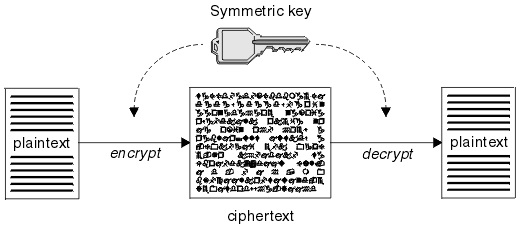
\includegraphics[width=0.7\textwidth]{abbildungen/symmetricEncoding.png}
	\centering
	\caption[
	Schaubild für eine symmetrische Verschlüsselung]{Schaubild für eine symmetrische Verschlüsselung\footnotemark}
	\label{fig:symmetricalEncoding}
\end{figure}
\footnotetext{\cite{Chapter211:online}}


Symmetrische Verschlüsselungsverfahren werden deshalb als sicher anerkannt, wenn man ohne den Schlüssel den Klartext nicht aus dem verschlüsselten Text ermitteln kann. \autocite[\pagef~5]{kryptographische_algorithmen}

\paragraph{\acf{DES}}\label{paragraph:data-encryption-standard}
\ac{DES}, oft auch \ac{DEA}, wurde 1975 im ''Federal Register'' der USA
veröffentlicht und als Kooperation zwischen dem \ac{NIST}, der \ac{NSA} und IBM entwickelt. \autocite[\pagef~232]{nsa-meyer}

\ac{DES} ist ein Blockchiffre-Verfahren, was bedeutet, dass die Daten in immer gleich großen Blöcken (bei \ac{DES} in Blöcken von 64 Zeichen) und mit einer immer gleichen Schlüssellänge (56 bit bei \ac{DES}) verschlüsselt werden. \autocite[\pagef~6]{kryptographische_algorithmen}

\paragraph{\acf{IDEA}}\label{paragraph:internet-datatencryption-algorithm}
\ac{IDEA} wurde 1990 als eine erweiterte Version zu \ac{DES} entwickelt und verwendet eine Schlüssellänge von 128 bit. \autocite[\pagef~6]{kryptographische_algorithmen}

\subsubsection[Asymmetrische Algorithmen und RSA-Verfahren]{Asymmetrische \glspl{algorithmus} und \acs{RSA}\nobreakdash Verfahren}\label{subsubsec:asymmetrische-algorithmen}
Asymmetrische Verschlüsselungsverfahren verwenden, im Gegensatz zu den symmetrischen Verschlüsselungsverfahren (\autoref{subsubsec:symmetrsiche-algorithmen}), zwei Schlüssel. Einen \gls{publicKey}, welcher zum Verschlüsseln der Daten verwendet wird und einen \gls{privateKey}, welcher zum Entschlüsseln der Daten verwendet wird. Wie der Name sagt, muss nur der private Key geheim gehalten werden.

Das \ac{RSA} ist das erste entwickelte \gls{publicKeyEncoding} und besitzt auch heute noch eine große Relevanz. \autocite[\pagef~168]{buchmann_einfuhrung_2016}

\paragraph[Schlüsselerzeugung]{Schlüsselerzeugung}\label{par:schluesselerzeugung}
Für die Erzeugung eines Schlüsselpaares für den \ac{RSA}"~\gls{algorithmus} werden einige Zahlen benötigt. Die Erste ist als Sicherheitsparameter eine Zahl \(k \in \mathbb{N}\), welche die Größe des Produktes der beiden für die Verschlüsselung gewählten Primzahlen angibt.. 
Zudem werden zwei, voneinander statistisch unabhängig, zufällige Primzahlen $p$ und $q$ gewählt, sodass der \ac{RSA} Modul $n$, der Wert, der später zum Ver- und Entschlüsseln genutzt wird, gebildet werden kann aus \(n = p*q\).
Zusätzlich wird eine natürliche Zahl $e$ gewählt, für die
\begin{equation}
    1 < e < \varphi(n) = (p - 1)(q - 1)\ \text{und}\ \gcd(e, (p-1)(q-1)) = 1
\end{equation}
gilt und daraus mit den folgenden Bedingungn
\begin{equation}
    1 < d < (p-1)(q-1)\ \text{und}\ d*e \equiv 1\mod(p-1)(q-1)
\end{equation}
eine weitere Zahl \(d \in \mathbb{N}\) gebildet.

Da $\gcd(e, (p-1)(q-1)) = 1$ ist, existiert eine solche Zahl $d$ definitiv. Berechnet werden kann sie mit dem \glspl{extendedEuklidAlgorithm}. Dabei ist zu beachten, dass $e$ stets ungerade ist. Der öffentliche Schlüssel bildet sich dabei aus dem Paar $(e, n)$ und der private Schlüssel aus der Zahl $d$. \autocite[\pagef~169]{buchmann_einfuhrung_2016}

Damit \ac{RSA} eine sichere Verschlüsselung garantieren kann, müssen die beiden Primzahlen $p$ und $q$ passend gewählt werden. Dafür ist es üblich, dass $k$ als gerade Zahl gewählt wird, die mittlerweile mindestens 1024-Bit lang ist. \autocite[\pagef~169]{buchmann_einfuhrung_2016}

\paragraph{Verschlüsselung}\label{par:verschluesselung}
Um mit dem \ac{RSA} \gls{algorithmus} eine Nachricht zu verschlüsseln, wird der öffentliche Schlüssel $(e, n)$ benötigt. Aus einem \gls{klartext} \(m \in \mathbb{Z}_m\) mit \(\mathbb{Z}_m\) als \ac{RSA} \gls{klartextraum} erhält man den verschlüsselten Text $c$ mit
\begin{equation}
    c = m^e\mod n
\end{equation}
$m$ kann wieder rekonstruiert werden mit
\begin{equation}
    m = c^d \mod n
\end{equation}
wobei $c$ der zuvor erhaltene verschlüsselte Text ist, $d$ ist der private Schlüssel und $n$ ist ein Teil des öffentlichen Schlüssels. \autocite[\pagef~6]{rsa-encryption}

\subsubsection[Hashfunktionen]{Hashfunktionen — \acf{SHA}}\label{subsubsec:hash-funktion}
Im Grundlegenden sind Hashfunktionen \glspl{algorithmus}, die einen Text beliebiger Länge zu einem neuen Text mit vorgegebener Länge komprimieren \autocite[\pagef~15]{anal_des_hash_function_2003}. Generiert werden sie mit Hilfe von sogenannten \glspl{compressfunc}.

Damit Hash- und \glspl{compressfunc} in der Kryptographie zur Authentifizierung, wie z.B. zur Speicherung von Passwörtern genutzt werden können, müssen noch ein paar Kritierien erfüllt werden. Diese werden folgend erklärt:

\begin{definition}
    Eine Einweghashfunktion ist eine Funktion $h$, die die folgenden Bedingungen erfüllt \autocite[\pagef~17]{anal_des_hash_function_2003}:    
    \begin{enumerate}
        \item Die Beschreibung von $h$ muss öffentlich bekannt sein und sollte keine geheimen Informationen erfordern (Erweiterung des Kerckhoff'schen Prinzips \autocite[]{petitcolas_information_nodate}).
        \item Das Argument $X$ kann von beliebiger Länge sein und das Ergebnis $h(X)$ hat eine feste Länge von $n$-Bits (mit $n \geq64$).
        \item Gegeben $h$ und $X$, muss die Berechnung von $h(X)$ einfach\footnotemark sein.
        \item Die Hashfunktion muss in dem Sinne monodirektional sein, dass es bei einem $Y$ im Abbild von $h$ schwer\footnotemark[\value{footnote}] ist, eine Nachricht $X$ zu finden, so dass $h(X)=Y$ ist, und dass es bei $X$ und $h(X)$ schwer\footnotemark[\value{footnote}] ist, eine Nachricht $X'\neq X$ zu finden, so dass $h(X') = h(X)$.
    \end{enumerate}
    \footnotetext{\enquote{einfach} und \enquote{schwer} sind hier im Kryptographischen Sinne zu verstehen und beziehen sich auf das Zusammenspiel von Laufzeit und Rechenaufwand eines \gls{algorithmus}}
\end{definition}

Da es nicht bekannt ist, ob es Einwegfunktionen gibt, die optimal arbeiten, werden in der Definition die Begriffe einfach und schwer verwendet, da es heutzutage noch keine \glspl{algorithmus} bekannt sind, die eine Einweghashfunktion schnell genug umkehren kann \autocite[\pagef~234]{buchmann_einfuhrung_2016}

Die \acfp{SHA} sind verschiedene kryptologische Hashfunktionen und eine modifizierte Version des \gls{MD5} (\acs{MD5}), welche zur Berechnung eines Prüfwertes für beliebige Nachrichten dienen und unter anderem die Grundlage zur Erstellung einer digitalen Signatur, genauer erläutert in \autoref{subsubsec:digitale-signaturen-und-zertifikate}, sind\autocite[]{WhatisSH81:online}.

2012 wurde \ac{SHA}-3 (auch bezeichnet als Keccak) von \ac{NIST} standardisiert und wird heute als sicher angesehen \autocite[\pagef~239]{buchmann_einfuhrung_2016}, aber auch die \glspl{algorithmus} unter \ac{SHA}-2 sind heute stark verbreitet. Unter \ac{SHA}-2 und \ac{SHA}-3 werden dabei nicht einzelne \glspl{algorithmus} sondern \gls{algorithmus}gruppen verstanden, deren zugrunde liegenden \glspl{algorithmus} sich primär in der Länge des Prüfwertes, den sie ausgeben unterscheiden. Häufig genutzt werden heute die \glspl{algorithmus} \ac{SHA}-256 und \ac{SHA}-512.

Da bei den \ac{SHA}-\glspl{algorithmus} selbst kleine Änderungen im \gls{klartext} schon für einen stark geänderten \gls{geheimtext}.
